\documentclass[a4paper,8pt,twocolumn]{article}
\usepackage[UTF8]{ctex}
\usepackage{graphicx}
\usepackage{fancyhdr}
\usepackage{amsmath}
\usepackage{subcaption}
\usepackage{float}
\usepackage[
  left=2cm,
  right=2cm,
  top=1.5cm,
  bottom=2.5cm
]{geometry}
\usepackage{siunitx}
\usepackage{booktabs}
\usepackage{enumitem}
\usepackage{array}
\usepackage{tabularx}
\newcolumntype{Y}{>{\centering\arraybackslash}X}
\usepackage{amssymb}
\usepackage{pgfplots}
\usepackage{pgfplotstable}
\pgfplotsset{compat=1.18}

%================ 标定曲线统一样式 ================
\pgfplotsset{
  calibplot/.style={
    width=0.92\columnwidth,
    height=0.22\textheight,
    scale only axis,
    grid=major,
    enlargelimits=false,
    xlabel={励磁电压 $U$ / V},
    ylabel={磁感应强度 $B$ / Gs},
    title style={font=\small},
    label style={font=\small},
    ticklabel style={font=\scriptsize},
    legend style={font=\scriptsize, at={(0.02,0.98)}, anchor=north west,
                  cells={anchor=west}}
  }
}
%=======================================================

\sisetup{
  per-mode=symbol,
  separate-uncertainty = true
}

\title{
  \textbf{\huge A-2：微波电子自旋共振}
}
\author{
  姓名~学号\\
  \small 中山大学物理学院~广东~广州
}

\pagestyle{fancy}
\fancyhf{}
\fancyhead[C]{A-2：微波电子自旋共振}
\fancyfoot[C]{\thepage}

\begin{document}
\maketitle

%%%%%%%%%%%%%%%%%%%%%%%%%%%%%%%%%%%%%%%%%%%%%%%%%%%%%%%%%%%%
\section{实验目的}

\begin{enumerate}
  \item 掌握微波段电子自旋共振（ESR）的实验方法；
  \item 了解微波电子自旋共振谱仪的结构与各微波器件的工作原理；
  \item 测定顺磁样品 DPPH 的朗德 $g$ 因子与共振线宽，并由线宽估算横向弛豫时间 $T_2$；
  \item 测量波导波长 $\lambda_g$ 并与理论值比较，对 TEMPO 样品进行同样的分析与对比讨论。
\end{enumerate}

%%%%%%%%%%%%%%%%%%%%%%%%%%%%%%%%%%%%%%%%%%%%%%%%%%%%%%%%%%%%
\section{实验仪器与装置}

FD-ESR-C 型微波电子自旋共振实验仪、数字式高斯计（含霍尔探头）、双踪示波器、电磁铁与扫描电源、样品（DPPH 与 TEMPO，固态粉末）。完整微波系统由左至右依次为：固态微波源、隔离器、环形器、双 T 调配器、吸收式谐振频率计、扭波导、矩形谐振腔与短路活塞。其矩形波导参数为 $a=\SI{22.86}{mm}$、$b=\SI{10.16}{mm}$。

%%%%%%%%%%%%%%%%%%%%%%%%%%%%%%%%%%%%%%%%%%%%%%%%%%%%%%%%%%%%
\section{实验原理}

\subsection{电子自旋共振条件}

具有总角动量 $\vec{P}_j$ 的电子，在恒定磁场 $\vec{B}_0$ 中获得塞曼能量
\begin{equation}
  E=-g\mu_B m_j B_0,\qquad m_j=\pm\tfrac{1}{2}
  \tag{A2.1}
\end{equation}
相邻能级间隔 $\Delta E=g\mu_B B_0$。在垂直于 $\vec{B}_0$ 方向施加角频率 $\omega$ 的微波交变磁场，当
\begin{equation}
  \hbar\omega = g\mu_B B_0,\quad\text{即}\quad \omega = \frac{g\mu_B}{\hbar}B_0
  \tag{A2.2}
\end{equation}
时发生共振跃迁，由此可反演样品的朗德因子
\begin{equation}
  g=\frac{h f}{\mu_B B_0}\tag{A2.3}
\end{equation}
DPPH 第二个氮原子上存在稳定的未成对自由电子，其轨道角动量已被淬灭，故 $g$ 接近自由电子值，参考值 $g_{\text{DPPH}}=2.0036$。

\subsection{波导与谐振腔}

矩形波导中 $\mathrm{TE}_{10}$ 模波长满足
\begin{equation}
  \lambda_g=\frac{\lambda}{\sqrt{1-(\lambda/\lambda_c)^2}},
  \quad \lambda_c=2a,\ \lambda=c/f
  \tag{A2.4}
\end{equation}
谐振腔长度为半波导波长整数倍 $l=P\lambda_g/2$ 时形成共振。改变短路活塞位置使相邻两次共振位置之差等于 $\lambda_g/2$，即可测得 $\lambda_g$。

\subsection{弛豫与线宽}

由 Bloch 方程，未达饱和的吸收信号为洛伦兹线型
\begin{equation}
  \chi''(\omega)\propto\frac{T_2}{1+(\omega-\omega_0)^2 T_2^2}
  \tag{A2.5}
\end{equation}
半高全宽为 $\Delta\omega_{1/2}=2/T_2$，对应磁场 FWHM
\begin{equation}
  T_2=\frac{2}{\gamma_e \Delta B_{1/2}}
  =\frac{2\hbar}{g\mu_B \Delta B_{1/2}}
  \tag{A2.6}
\end{equation}
其中 $\gamma_e=g\mu_B/\hbar$ 为旋磁比。

\subsection{对实验装置的理解}

实验装置最左端产生微波。双 T 接头的 E 臂、H 臂分别调节竖直方向电场与水平方向磁场以匹配相位；CH2 接收的是空间驻波某一点处的功率。该实验的巧妙之处在于：电子的共振是难以直接观察的微观变化，实验先令微波在波导内形成驻波，再施加随时间变化的扫描磁场，当某一时刻磁场满足共振条件时，样品（可视作一个相位改变器）使腔内驻波相位发生改变，从而使固定位置处的检波功率发生变化；由扫描磁场的瞬时取值即可对应到共振磁场。整个过程将微观的吸收放大为宏观可观测的功率变化，实现了"以驻波放大共振"的核心思想。

%%%%%%%%%%%%%%%%%%%%%%%%%%%%%%%%%%%%%%%%%%%%%%%%%%%%%%%%%%%%
\section{实验内容与步骤}

实验分两次进行，每次开始前均完成磁场\,--\,励磁电压标定。具体步骤如下：

\begin{enumerate}[label=(\arabic*)]
  \item 连接主机、微波系统、电磁铁与示波器，预热 20 min。霍尔探头置于谐振腔磁场空隙中心。
  \item 调节励磁电源电位器，由 $U=0$ 至 $\SI{5.0}{V}$ 以 $\Delta U=\SI{0.2}{V}$ 步进，记录高斯计示数 $B$，作 $B$\,--\,$U$ 线性拟合。
  \item 移开高斯探头放入样品，扫描电源调到较大值，调节双 T 调配器，使示波器上信号跳动出现共振。
  \item 将示波器输入通道接到直流 DC 档，调节双 T 调配器使 DC 信号最大，调短路活塞使 DC 信号最小；再切到 $\SI{5}{mV}$ 或 $\SI{10}{mV}$ 交流档观察共振。微调双 T 及短路活塞使信号最强，细调励磁电源使两个共振峰均匀出现（两相位）。
  \item 记录共振时励磁电压 $U_{\text{res}}$ 与微波频率 $f$（多次读数）；由标定公式反推 $B_0$，由式 (A2.3) 计算 $g$。
  \item 移动短路活塞分别在三个相邻共振位 $L_1$、$L_2$、$L_3$ 处读数，由 $\lambda_g/2 = L_i - L_{i+1}$ 计算波导波长，并与式 (A2.4) 理论值比较。
  \item 切换示波器至 X-Y 显示方式，由调节励磁电源使吸收峰水平移动一格，记录电压变化 $\Delta U_{1\text{div}}$；读出吸收峰半高宽对应的格数，由标定斜率换算为 $\Delta B_{1/2}$，代入式 (A2.6) 计算 $T_2$。
  \item 将样品由 DPPH 更换为 TEMPO，重复 (4)\,$\sim$\,(7)，作完全相同的测试与分析。
\end{enumerate}

\noindent\textbf{操作中的观察}：实验进行两次标定。实验操作中，将霍尔传感器放入样品位时，应使"板"与导波管的方向平行，才能使高斯计的示数最大。实验过程中 CH2 信号并非完全对称，波的底部可能出现不光滑的变化；在缩小扫描电源后该问题得到缓解，CH1 图形也更加光滑。可以认为扫描电源过大会使扫描信号不稳、出现失真；若希望 X-Y 中高斯吸收波形完整显示，应尽量使用较小的扫描电源电压。

%%%%%%%%%%%%%%%%%%%%%%%%%%%%%%%%%%%%%%%%%%%%%%%%%%%%%%%%%%%%
\section{实验结果与分析}
\label{sec:results}

\subsection{磁场强度--励磁电压标定}

两次实验前分别进行了 26 点的 $B$\,--\,$U$ 标定。原始数据见数据记录文件，拟合结果如图\,\ref{fig:calib1}\,与图\,\ref{fig:calib2}\,所示。

\begin{figure}[H]
  \centering
  \begin{tikzpicture}
  \begin{axis}[calibplot,title={第一次标定（DPPH 第一组）},
    legend entries={实测数据, 线性拟合}]
    \addplot[only marks,mark=o,mark size=1pt,blue] coordinates {
      (0,3217)(0.2,3223)(0.4,3229)(0.6,3235)(0.8,3241)(1.0,3247)(1.2,3252)
      (1.4,3258)(1.6,3264)(1.8,3269)(2.0,3275)(2.2,3280)(2.4,3286)(2.6,3292)
      (2.8,3297)(3.0,3303)(3.2,3309)(3.4,3314)(3.6,3320)(3.8,3326)(4.0,3331)
      (4.2,3337)(4.4,3343)(4.6,3348)(4.8,3354)(5.0,3360)};
    \addplot[red,thick,domain=0:5.0] {28.21*x+3218.5};
  \end{axis}
  \end{tikzpicture}
  \caption{第一次磁场标定及线性拟合：$B_1=28.21\,U+3218.5$，$R^2>0.999$}
  \label{fig:calib1}
\end{figure}

\begin{figure}[H]
  \centering
  \begin{tikzpicture}
  \begin{axis}[calibplot,title={第二次标定（DPPH 第二组及 TEMPO）},
    legend entries={实测数据, 线性拟合}]
    \addplot[only marks,mark=o,mark size=1pt,blue] coordinates {
      (0,3197)(0.2,3203)(0.4,3208)(0.6,3214)(0.8,3220)(1.0,3225)(1.2,3231)
      (1.4,3236)(1.6,3242)(1.8,3247)(2.0,3253)(2.2,3258)(2.4,3264)(2.6,3269)
      (2.8,3275)(3.0,3280)(3.2,3286)(3.4,3292)(3.6,3297)(3.8,3303)(4.0,3308)
      (4.2,3314)(4.4,3319)(4.6,3325)(4.8,3330)(5.0,3336)};
    \addplot[red,thick,domain=0:5.0] {27.73*x+3197.3};
  \end{axis}
  \end{tikzpicture}
  \caption{第二次磁场标定及线性拟合：$B_2=27.73\,U+3197.3$，$R^2>0.999$}
  \label{fig:calib2}
\end{figure}

\noindent 两次标定的斜率差异约 $1.7\%$，主要来自电磁铁剩磁与初始状态不同。后续将分别采用相应公式由 $U_{\text{res}}$ 反推 $B_0$。

\subsection{共振信号与 $g$ 因子}

在双 T 调配相位 1 和相位 2 两种状态下分别记录了 DPPH 的稳定共振信号，如图\,\ref{fig:dpph_res}\,所示。两相位下共振位置一致，仅信号形态略有差异，说明双 T 调节主要改变载波相位而不影响共振条件。

\begin{figure}[H]
  \centering
  \begin{subfigure}{0.48\columnwidth}
    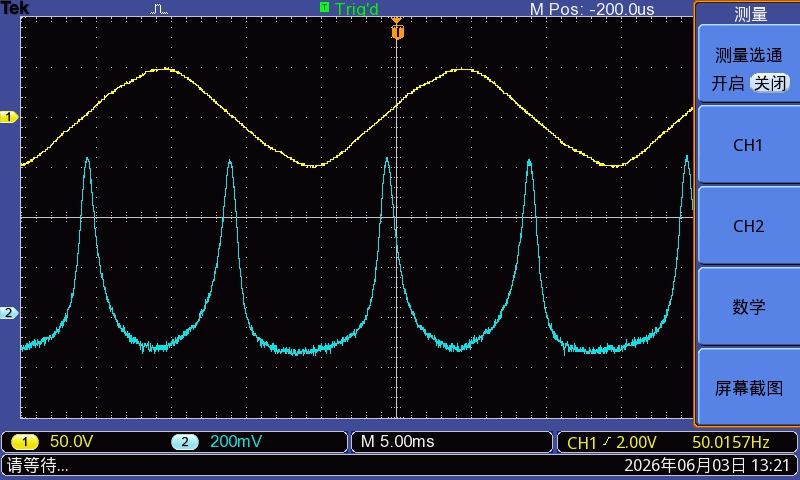
\includegraphics[width=\linewidth]{DPPH共振信号_相位1.JPG}
    \caption{相位 1}
  \end{subfigure}\hfill
  \begin{subfigure}{0.48\columnwidth}
    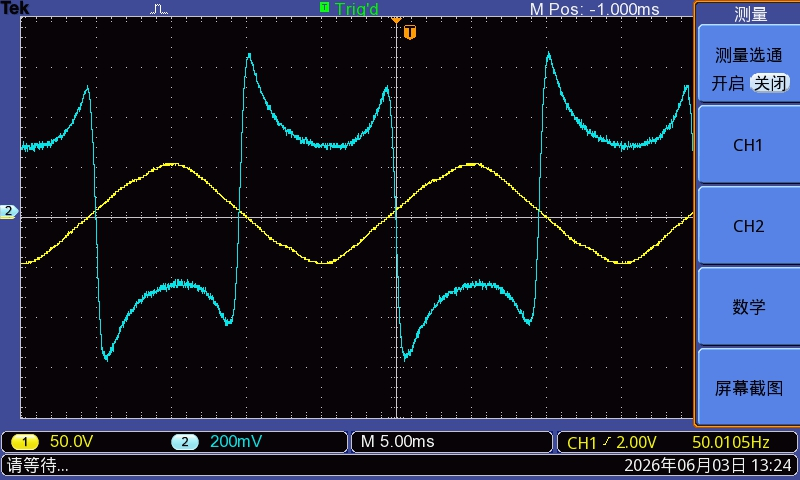
\includegraphics[width=\linewidth]{DPPH共振信号_相位2.JPG}
    \caption{相位 2}
  \end{subfigure}
  \caption{DPPH 共振信号（示波器交流档观察）}
  \label{fig:dpph_res}
\end{figure}

实测共振电压与频率（频率计三次读数）见表\,\ref{tab:res}。

\begin{table}[H]
\centering
\caption{DPPH 与 TEMPO 共振参数}
\label{tab:res}
\small
\begin{tabular}{lccc}
\toprule
样品 & $U_{\text{res}}$ / V & $f$ / GHz & 所用标定 \\
\midrule
DPPH (1) & 4.61 & 9.3750 & 第一次 \\
DPPH (2) & 4.98 & 9.3775 & 第二次 \\
TEMPO    & 5.05 & 9.3765 & 第二次 \\
\bottomrule
\end{tabular}
\end{table}

由对应标定公式得共振磁感应强度：
\begin{equation*}
\begin{aligned}
B_{0,\text{DPPH}}^{(1)} &= 28.21\!\times\!4.61+3218.5 = \SI{3348.6}{Gs}\\
B_{0,\text{DPPH}}^{(2)} &= 27.73\!\times\!4.98+3197.3 = \SI{3335.4}{Gs}\\
B_{0,\text{TEMPO}}      &= 27.73\!\times\!5.05+3197.3 = \SI{3337.3}{Gs}
\end{aligned}
\end{equation*}

代入式 (A2.3)（$h=\SI{6.626e-34}{J\cdot s}$，$\mu_B=\SI{9.274e-24}{J/T}$）：
\begin{equation*}
g_{\text{DPPH}}^{(1)}=\frac{hf}{\mu_B B_0}=2.00048,\quad g_{\text{DPPH}}^{(2)}=2.0086
\end{equation*}
\begin{equation*}
\bar{g}_{\text{DPPH}}=2.0046\pm 0.0042,\quad g_{\text{TEMPO}}=2.0073
\end{equation*}

DPPH 的实验均值 $\bar{g}=2.0046$ 与参考值 $2.0036$ 在不确定度范围内一致；TEMPO 实测略偏高，文献参考值约 $2.0060$，符合自由基类样品的一般范围。

\subsection{微波频率与波导波长}

\subsubsection*{微波频率}

频率计三次读数为 $9.3750$、$9.3775$、$9.3765$ GHz：
\begin{equation*}
\bar{f}=9.3763~\text{GHz},\quad s_f=\SI{0.00126}{GHz}
\end{equation*}
A 类不确定度 $u_A(\bar{f})=s_f/\sqrt{3}=\SI{0.00073}{GHz}$；频率计分辨率取 $\SI{1}{MHz}$，$u_B=\SI{0.58}{MHz}$，合成 $u(f)\approx\SI{0.93}{MHz}$。故
\begin{equation*}
f=(9.3763\pm 0.0009)\,\text{GHz}
\end{equation*}

\subsubsection*{波导波长测量}

短路活塞三个相邻谐振位置 $L_1=\SI{52.730}{mm}$，$L_2=\SI{30.450}{mm}$，$L_3=\SI{7.795}{mm}$，给出两个半波长测量：
\begin{equation*}
d_1=L_1-L_2=\SI{22.280}{mm},\ d_2=L_2-L_3=\SI{22.655}{mm}
\end{equation*}
均值 $\bar d=\SI{22.4675}{mm}$，故 $\lambda_g=2\bar d=\SI{44.94}{mm}$。

\noindent\textbf{不确定度分析}：A 类——样本标准差
\begin{equation*}
s_d=\sqrt{\sum(d_i-\bar d)^2/(n-1)}=\SI{0.265}{mm}
\end{equation*}
均值标准差 $u_A(\bar d)=s_d/\sqrt{n}=\SI{0.188}{mm}$。B 类——活塞螺旋读数误差 $\Delta=\SI{0.01}{mm}$，$u_B=\Delta/\sqrt{3}=\SI{0.006}{mm}$，可忽略。故
\begin{equation*}
u(\bar d)=\SI{0.188}{mm},\quad u(\lambda_g)=2u(\bar d)=\SI{0.38}{mm}
\end{equation*}
\begin{equation*}
\boxed{\lambda_g=(44.94\pm 0.38)\,\text{mm}=(4.494\pm 0.038)\!\times\!10^{-2}\,\text{m}}
\end{equation*}

\subsubsection*{理论值比较}

$\lambda_c=2a=\SI{45.72}{mm}$，$\lambda=c/\bar{f}=\SI{31.97}{mm}$，由式 (A2.4)：
\begin{equation*}
\lambda_g^{\text{th}}=\frac{31.97}{\sqrt{1-(31.97/45.72)^2}}=\SI{44.78}{mm}
\end{equation*}
理论值 $\lambda_g^{\text{th}}=\SI{44.78}{mm}$ 落入实验区间 $(44.56,45.32)$ mm 内，与实验值的相对偏差仅 $0.36\%$，二者高度吻合，验证了 $\mathrm{TE}_{10}$ 模波导色散关系。

\subsection{线宽测量与弛豫时间}

X-Y 显示方式下，调整励磁电源使吸收峰水平移动一格所需电压差为 $\Delta U_{1\text{div}}=\SI{0.138}{V}$。由此可将吸收峰半高宽换算为磁场宽度。DPPH 与 TEMPO 的 X-Y 谱线（即"磁场强度\,--\,功率"曲线）在两个相位下的实测图像如图\,\ref{fig:dpph_xy}\,与图\,\ref{fig:tempo_xy}\,所示。

\begin{figure}[H]
  \centering
  \begin{subfigure}{0.48\columnwidth}
    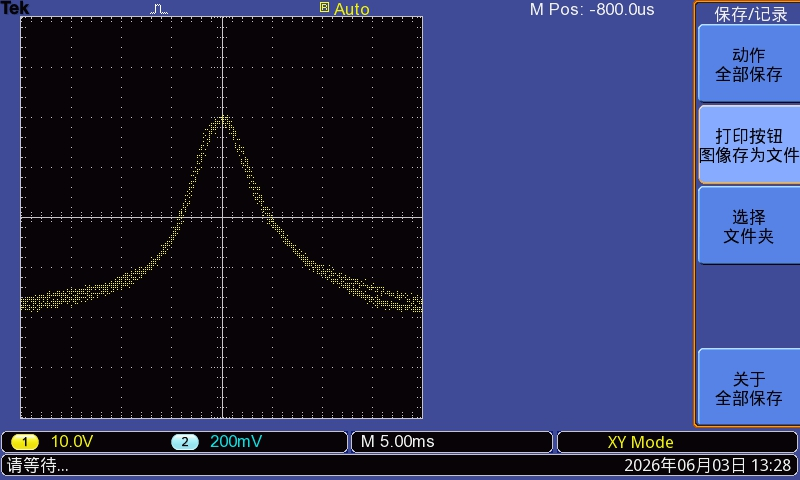
\includegraphics[width=\linewidth]{DPPH磁场强度-功率_相位1.JPG}
    \caption{相位 1}
  \end{subfigure}\hfill
  \begin{subfigure}{0.48\columnwidth}
    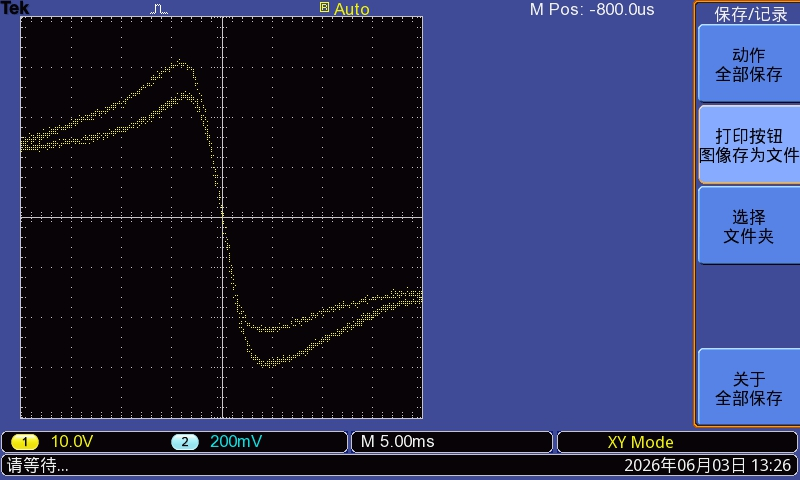
\includegraphics[width=\linewidth]{DPPH磁场强度-功率_相位2.JPG}
    \caption{相位 2}
  \end{subfigure}
  \caption{DPPH 磁场强度\,--\,功率曲线（X-Y 模式）}
  \label{fig:dpph_xy}
\end{figure}

\begin{figure}[H]
  \centering
  \begin{subfigure}{0.48\columnwidth}
    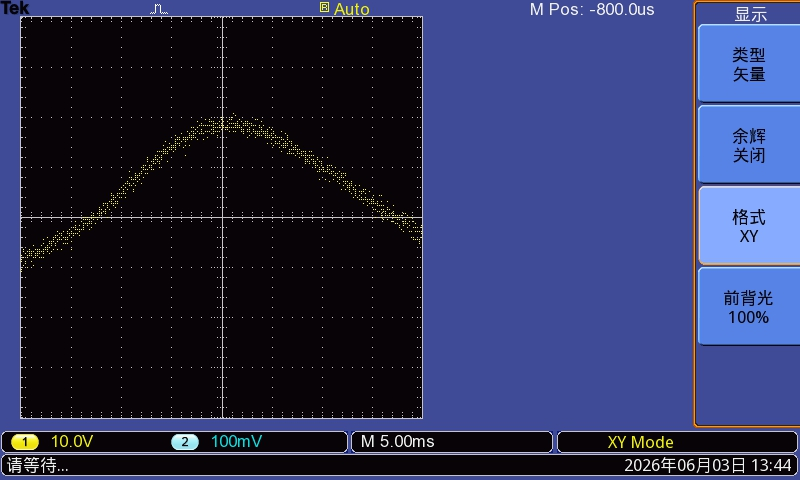
\includegraphics[width=\linewidth]{TEMPO磁场强度-功率_相位1.JPG}
    \caption{相位 1}
  \end{subfigure}\hfill
  \begin{subfigure}{0.48\columnwidth}
    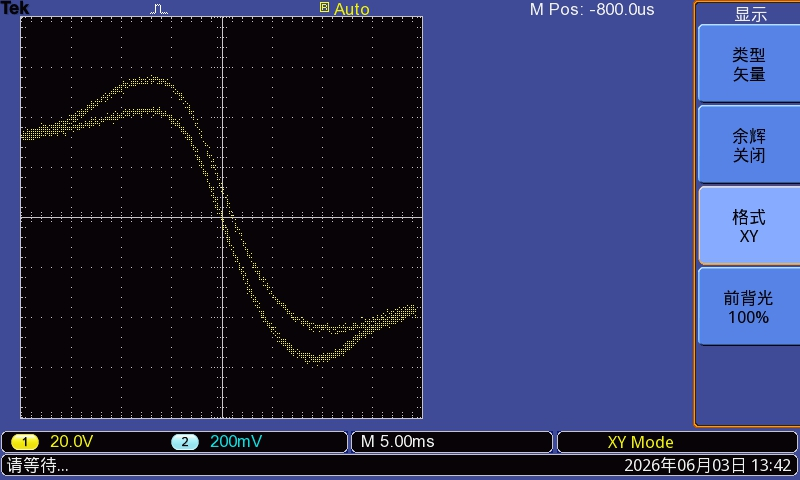
\includegraphics[width=\linewidth]{TEMPO磁场强度-功率_相位2.JPG}
    \caption{相位 2}
  \end{subfigure}
  \caption{TEMPO 磁场强度\,--\,功率曲线（X-Y 模式）}
  \label{fig:tempo_xy}
\end{figure}

读数结果：DPPH 半高宽 $1.6$ 格，TEMPO 半高宽 $6$ 格。换算到电压宽度
\begin{equation*}
\Delta U_{\text{DPPH}}=1.6\!\times\!0.138=\SI{0.221}{V}
\end{equation*}
\begin{equation*}
\Delta U_{\text{TEMPO}}=6\!\times\!0.138=\SI{0.828}{V}
\end{equation*}
按第二次标定斜率 $k_2=\SI{27.73}{Gs/V}$ 转化为磁场半高宽：
\begin{equation*}
\Delta B_{\text{DPPH}}=k_2\Delta U_{\text{DPPH}}=\SI{6.12}{Gs}=\SI{6.12e-4}{T}
\end{equation*}
\begin{equation*}
\Delta B_{\text{TEMPO}}=k_2\Delta U_{\text{TEMPO}}=\SI{22.96}{Gs}=\SI{22.96e-4}{T}
\end{equation*}

由式 (A2.6)，$\gamma_e=g\mu_B/\hbar=\SI{1.760e11}{rad/(s\cdot T)}$（取 $g\approx 2.0048$）：
\begin{equation*}
T_2^{\text{DPPH}}=\frac{2}{\gamma_e\Delta B_{\text{DPPH}}}=\SI{1.85e-8}{s}\approx\SI{18.5}{ns}
\end{equation*}
\begin{equation*}
T_2^{\text{TEMPO}}=\frac{2}{\gamma_e\Delta B_{\text{TEMPO}}}=\SI{4.94e-9}{s}\approx\SI{4.94}{ns}
\end{equation*}

DPPH 测得 $T_2$ 与文献 $\sim$10\,--\,60 ns 量级一致；TEMPO 由于固态下分子间偶极\,--\,偶极相互作用强烈，造成线宽显著增大、$T_2$ 显著缩短。

\subsection{附加讨论：仪器线宽的量化建模}

将上述线宽结果与文献参考值比较：纯 DPPH 的本征 FWHM 约为 $\SI{2.7}{Gs}$，而本实验测得 $\Delta B_{\text{DPPH}}^{\text{obs}}=\SI{6.12}{Gs}$，明显偏大；固态 TEMPO 的本征 FWHM 文献典型值约 $\SI{25}{Gs}$，实测 $\Delta B_{\text{TEMPO}}^{\text{obs}}=\SI{22.96}{Gs}$ 反而略偏小。两样品的偏离方向相反，提示其成因并不相同。

观测线型为样品本征线型与仪器响应函数的卷积，无论 Lorentzian 还是 Gaussian 卷积，其 FWHM 都只能随之增大而不能减小，即对任一样品恒有 $\Delta B^{\text{obs}}\geq \Delta B^{\text{int}}$。据此可对两样品的偏离方向分别给出诊断：DPPH 实测偏大与卷积加宽规律一致，多出的 $\sim\SI{3.4}{Gs}$ 应归因于仪器响应；TEMPO 实测反而偏小，与卷积"只增不减"的约束相悖，说明所采用的文献参考值并非真正的样品本征值——其测量本身可能已含较宽的仪器贡献，亦可能我方样品因制备条件（粒度、纯度、是否顺磁稀释、温度等）与文献样品有别，本征线宽本身就较小，甚至不排除存在样品内部的交换窄化或局部分子运动等动力学效应。无论何种原因，TEMPO 的偏离都不应归咎于仪器。

综合两样品的诊断，可推断仪器线宽 $\Delta B_{\text{inst}}$ 满足
\begin{equation*}
  \Delta B_{\text{DPPH}}^{\text{int}}<\Delta B_{\text{inst}}<\Delta B_{\text{TEMPO}}^{\text{int}}
\end{equation*}
即仪器贡献处于两样品本征线宽之间：DPPH 实测线宽主要由仪器响应主导，TEMPO 实测则主要反映样品本征线宽，仪器仅作小量修正。

在此基础上可建立简单的仪器线宽反演模型。若仪器响应与样品本征均近似为 Lorentzian，则二者卷积仍为 Lorentzian，FWHM 线性相加：
\begin{equation}
  \Delta B^{\text{obs}}=\Delta B^{\text{int}}+\Delta B^{\text{inst}}
  \tag{A2.7}
\end{equation}
取 DPPH 为窄线标样，代入文献本征值得
\begin{equation*}
\Delta B_{\text{inst}}^{\text{Lor}}=\Delta B_{\text{DPPH}}^{\text{obs}}-\Delta B_{\text{DPPH}}^{\text{int}}\approx 6.12-2.7=\SI{3.4}{Gs}
\end{equation*}
若展宽主要源于高斯型机制（如调制磁场幅度、磁场不均匀等），则 FWHM 按平方相加：
\begin{equation}
  (\Delta B^{\text{obs}})^2=(\Delta B^{\text{int}})^2+(\Delta B^{\text{inst}})^2
  \tag{A2.8}
\end{equation}
\begin{equation*}
\Delta B_{\text{inst}}^{\text{Gau}}=\sqrt{6.12^2-2.7^2}\approx\SI{5.5}{Gs}
\end{equation*}
两模型给出的仪器线宽估计在 $\SI{3.4}{Gs}\sim\SI{5.5}{Gs}$ 之间。将其代回 TEMPO 反推本征线宽，得 $\Delta B_{\text{TEMPO}}^{\text{int}}\approx\SI{19.6}{Gs}\sim\SI{22.3}{Gs}$，仍小于文献 $\SI{25}{Gs}$，进一步印证了前述对 TEMPO 偏小成因的诊断——其根源在于样品/文献差异，而非仪器贡献。

该模型尚有以下局限。其一，真实 ESR 线型多为 Voigt 型，应采用 Faddeeva 函数对吸收线进行 Voigt 拟合，方可同时分离 Lorentzian 与 Gaussian 两路贡献并得到更可靠的仪器线宽；其二，仪器线宽本身随调制幅度、扫描速率与微波功率变化，需对多组工况测量同一标样以建立 $\Delta B_{\text{inst}}(B_{\text{mod}},f_{\text{mod}},P_{\mu w})$ 的经验关系；其三，目前以 DPPH 文献本征值作为"参考"存在循环论证的风险（文献本征值本身亦由有限分辨率的仪器测得），更严谨的做法是引入超窄线宽标样（如稀溶液 DPPH/苯，FWHM $<\SI{1}{Gs}$）独立标定仪器，再以此修正其他样品的实测线宽并扣除仪器贡献。

%%%%%%%%%%%%%%%%%%%%%%%%%%%%%%%%%%%%%%%%%%%%%%%%%%%%%%%%%%%%
\clearpage
\onecolumn
\section*{参考文献}

\begin{enumerate}[label={[\arabic*]}]
  \item 杨福家. 原子物理学[M]. 5 版. 北京: 高等教育出版社, 2019.
  \item 熊俊. 近代物理实验[M]. 北京: 北京师范大学出版社, 2017.
  \item Weil J A, Bolton J R. Electron Paramagnetic Resonance: Elementary Theory and Practical Applications[M]. 2nd ed. Hoboken: Wiley-Interscience, 2007.
  \item Poole C P. Electron Spin Resonance: A Comprehensive Treatise on Experimental Techniques[M]. 2nd ed. New York: Dover, 1996.
  \item 戴道生. 铁磁学[M]. 2 版. 北京: 科学出版社, 2017.
  \item Krzystek J, Sienkiewicz A, Pardi L, et al. DPPH as a Standard for High-field EPR[J]. \textit{Journal of Magnetic Resonance}, 1997, 125(1): 207--211.
\end{enumerate}

\clearpage

\section{教师签名页}
  \begin{figure}[H]
  \centering
  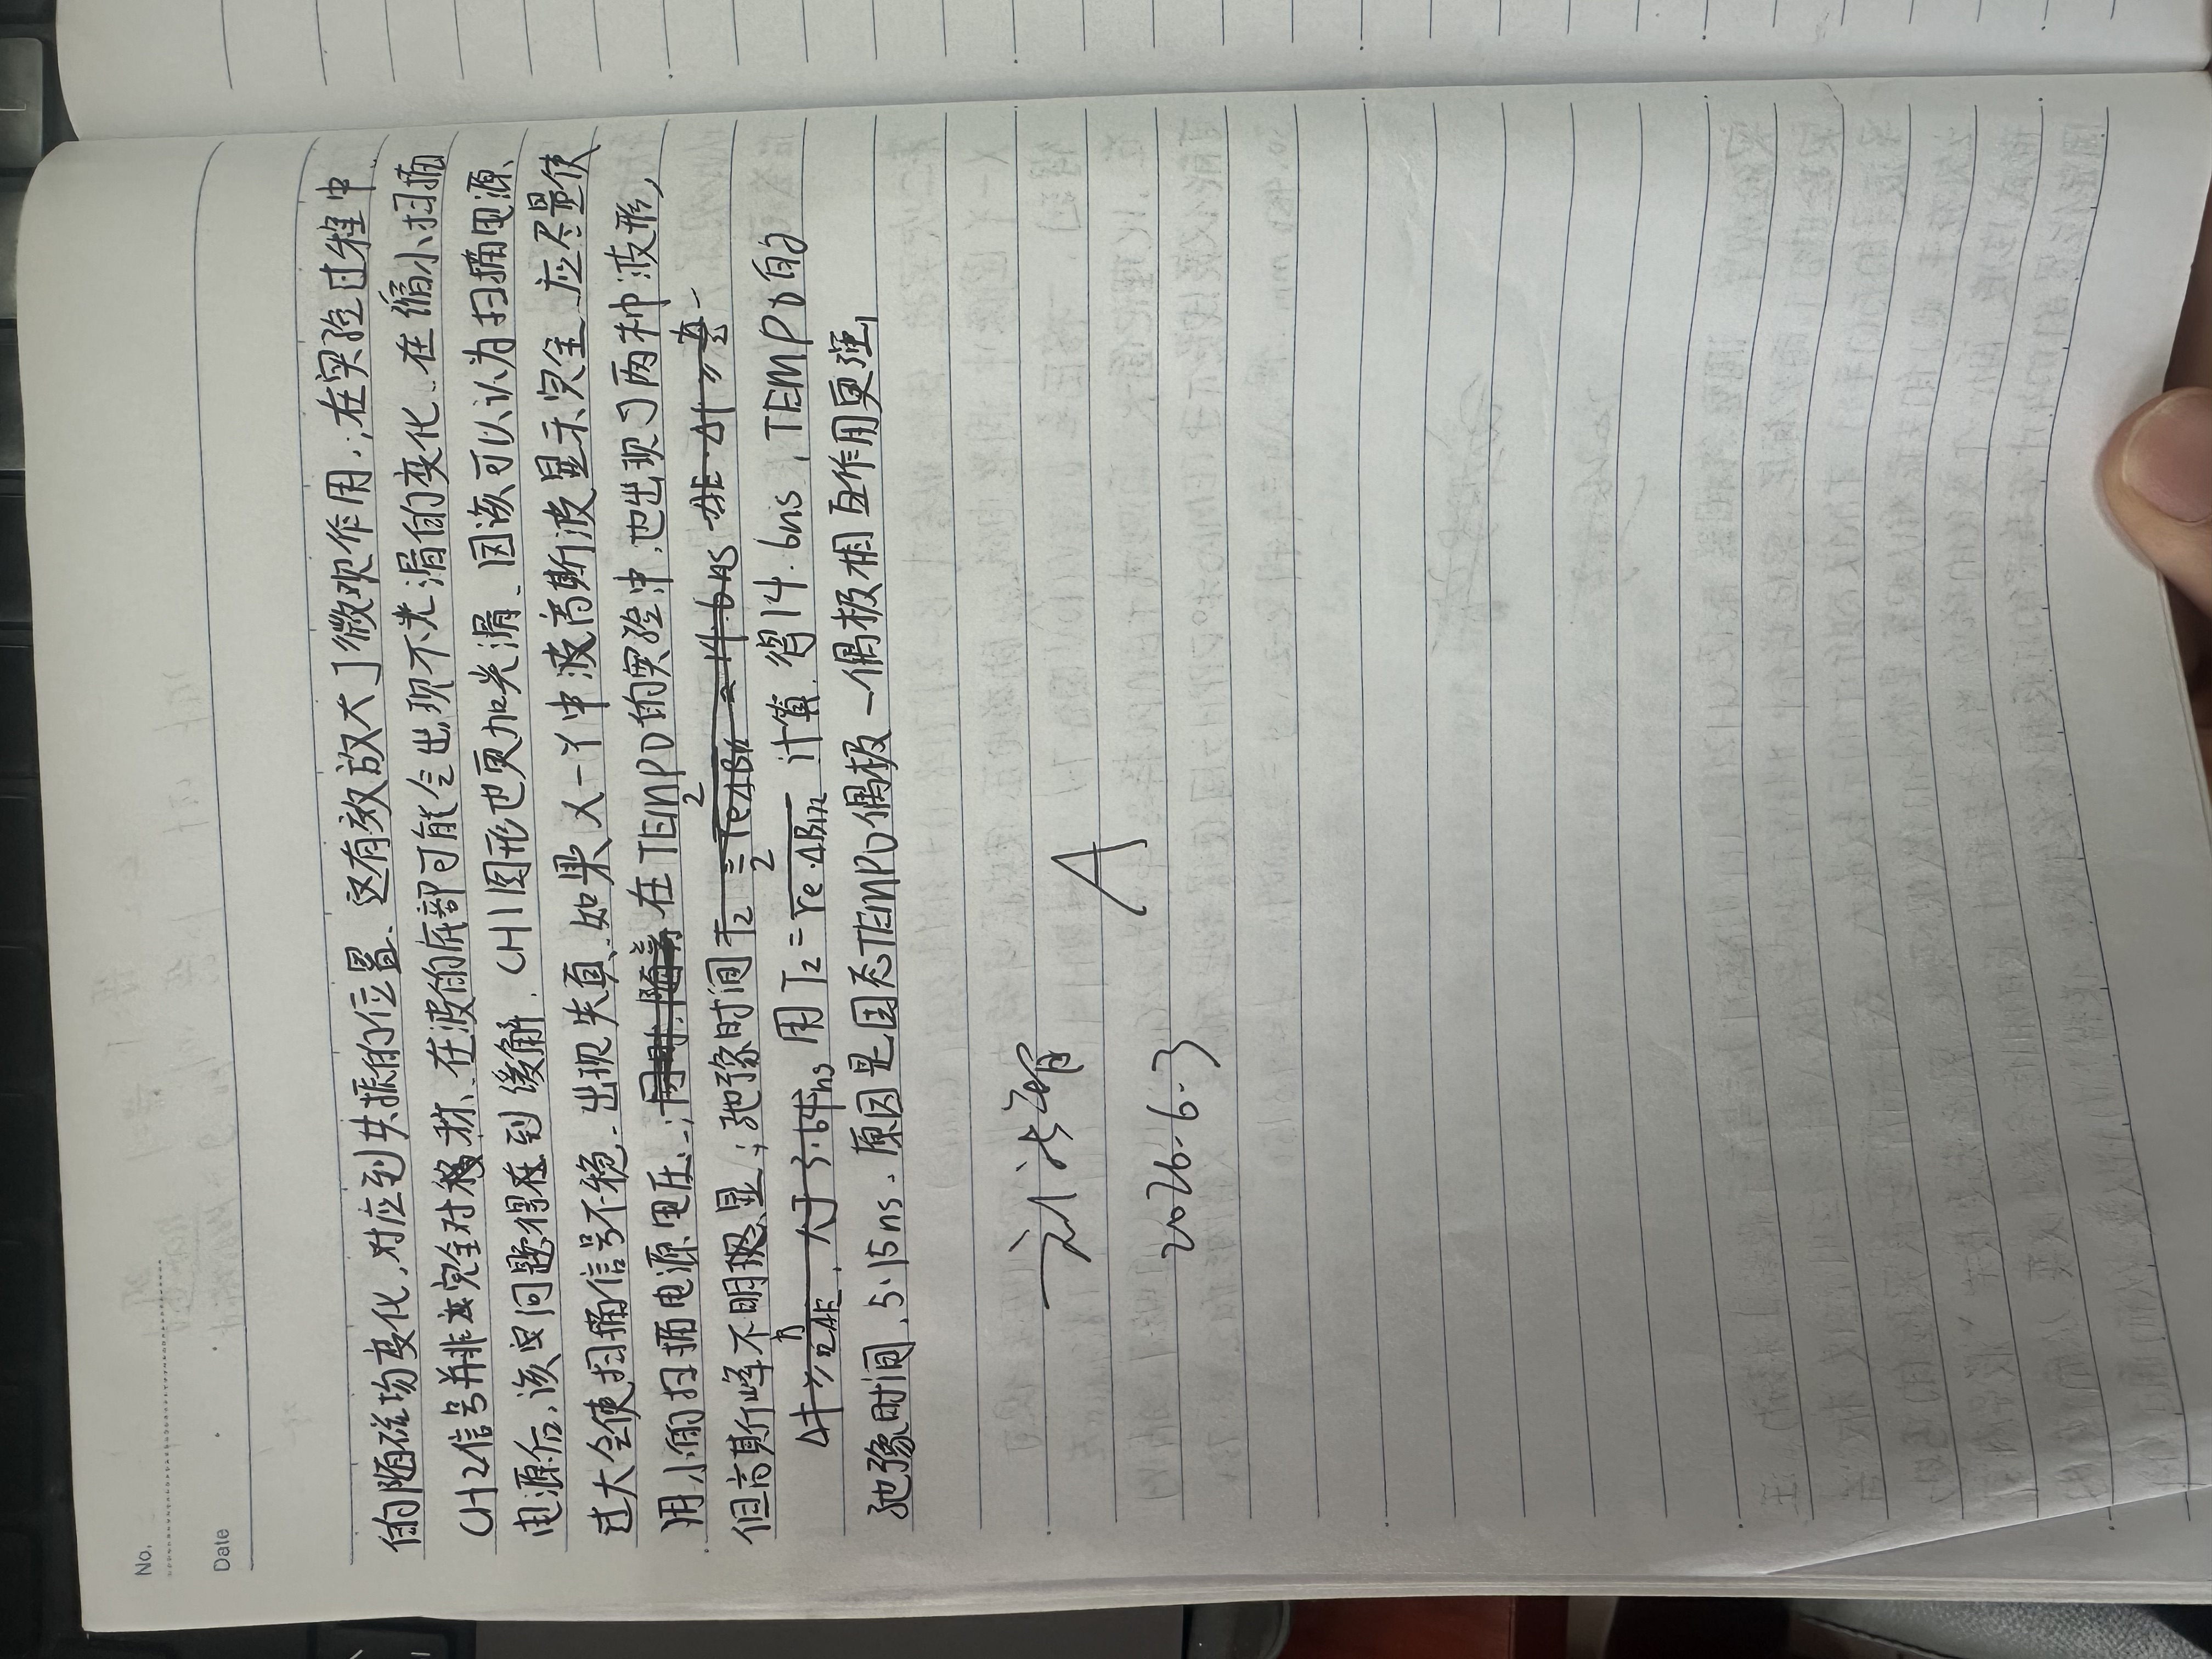
\includegraphics[width=0.85\columnwidth]{签名页.jpeg}
  \caption{教师签名页}
  \end{figure}

\end{document}
